\documentclass[aspectratio=169,10pt]{beamer}

% ==========================================================================
% THEME SETUP
% ==========================================================================

\usepackage{comment}

% Queen's University colors
\definecolor{QueensBlue}{HTML}{002452}
\definecolor{QueensRed}{HTML}{B90E31}
\definecolor{QueensGold}{HTML}{FABD0F}

\usetheme{default}
\setbeamertemplate{navigation symbols}{}
\setbeamertemplate{itemize items}{\textbullet}
\usefonttheme[onlymath]{serif}
\setbeamersize{text margin left=0.75cm, text margin right=0.75cm}

% Colors
\setbeamercolor{frametitle}{fg=QueensRed}
\setbeamercolor{title}{fg=QueensGold}
\setbeamercolor{author}{fg=QueensGold}
\setbeamercolor{institute}{fg=QueensGold!80}
\setbeamercolor{date}{fg=QueensGold!80}
\setbeamercolor{structure}{fg=QueensBlue}
\setbeamercolor{block title}{fg=white, bg=QueensBlue}
\setbeamercolor{block body}{bg=QueensBlue!5}
\setbeamercolor{alerted text}{fg=QueensRed}
\setbeamercolor{section in head/foot}{fg=white, bg=QueensBlue}
\setbeamercolor{section in head/foot shaded}{fg=QueensBlue!40, bg=QueensBlue}

% Frame title
\setbeamerfont{frametitle}{size=\Large, series=\bfseries}
\setbeamertemplate{frametitle}{\vspace{0.25cm}\insertframetitle\par}

% Tri-color bar for normal frames (headline)
\setbeamertemplate{headline}{%
  \noindent\hbox to\paperwidth{%
    {\color{QueensBlue}\vrule height4pt width0.36\paperwidth}%
    {\color{QueensGold}\vrule height4pt width0.28\paperwidth}%
    {\color{QueensRed}\vrule height4pt width0.36\paperwidth}%
  }%
}

% Footline: section navigation
\setbeamertemplate{footline}{%
  \begin{beamercolorbox}[wd=\paperwidth, ht=2.5ex, dp=1.125ex]{section in head/foot}%
    \hfill\insertsectionnavigationhorizontal{0.95\paperwidth}{}{\hfill}\hfill%
  \end{beamercolorbox}%
}

% Section divider: colored background + centered white title
\newcommand{\sectionslide}[2]{%
  \begingroup
  \setbeamercolor{background canvas}{bg=#1}
  \begin{frame}[plain,c]
    \centering{\Huge\bfseries\color{white}#2}
  \end{frame}
  \endgroup
}

% ==========================================================================
% PACKAGES AND MACROS
% ==========================================================================

\usepackage{amsmath,amssymb}
\PassOptionsToPackage{hyphens}{url}
\usepackage{hyperref}
\urlstyle{same}
\usepackage{booktabs}
\usepackage{array}
\usepackage{graphicx}
\usepackage{tikz}
\usetikzlibrary{arrows.meta, positioning, fit, backgrounds, calc}

\graphicspath{{../thesis/figures/}{../thesis/figures/raw/}{figures/}{figures/ppt/}}

\newcommand{\source}[1]{\vfill{\tiny\color{gray}#1\par}}
\newcommand{\R}{\mathbb{R}}
\newcommand{\E}{\mathbb{E}}
\newcommand{\DSQ}{\mathrm{DSQ}}
\newcommand{\clip}{\mathrm{clip}}

% ==========================================================================
% METADATA
% ==========================================================================

\title[Toward Visually Robust Quadruped Parkour]{Toward Visually Robust Quadruped Parkour\\via Monocular Depth Estimation}
\subtitle{An experimental study of monocular depth for quadruped parkour}
\author[Theo Lemay]{Theo Lemay\\\small MTHE 499 Thesis}
\institute[Queen's]{Queen's University\\\small Supervisor: Prof.\ Joshua Marshall}
\date{April 2026}

\begin{document}

% ==========================================================================
% TITLE SLIDE
% ==========================================================================
{
\setbeamercolor{background canvas}{bg=QueensBlue}
\setbeamerfont{title}{size=\LARGE, series=\bfseries}
\setbeamercolor{title}{fg=white}
\setbeamercolor{subtitle}{fg=QueensGold}
\setbeamercolor{author}{fg=white}
\setbeamercolor{institute}{fg=QueensGold!80}
\setbeamercolor{date}{fg=QueensGold!80}
\begin{frame}[plain,c]
  \titlepage
\end{frame}
}

% ==========================================================================
\section{Problem}
% ==========================================================================

\sectionslide{QueensRed}{Problem}

% Script:
% - Open with the deployment gap: most parkour papers assume a depth camera at test time.
% - My question was whether a pretrained monocular depth model can provide the right geometry instead.
% - The contribution is experimental and methodological: what I tried, what worked, what failed, and what that rules out.
% - Transition: before the experiments, I need a clean mathematical model of the task.
\begin{frame}{Problem and Thesis Question}
  \begin{columns}[T,onlytextwidth]
    \column{0.57\textwidth}
    \begin{itemize}
      \item Vision-based quadruped parkour usually deploys with an onboard \alert{depth camera}.
      \item On Go2-class platforms, \alert{perception} is the bottleneck: deployment is easier from RGB than from specialized depth hardware.
      \item I explored \alert{monocular depth as a canonical representation}, instead of relying on photorealistic rendering or heavy visual domain randomization.
    \end{itemize}

    \vspace{0.5em}
    \begin{block}{Thesis Question}
      Can a pretrained monocular depth estimator preserve enough terrain geometry for a distilled parkour policy to act reliably?
    \end{block}

    \column{0.39\textwidth}
    \centering
    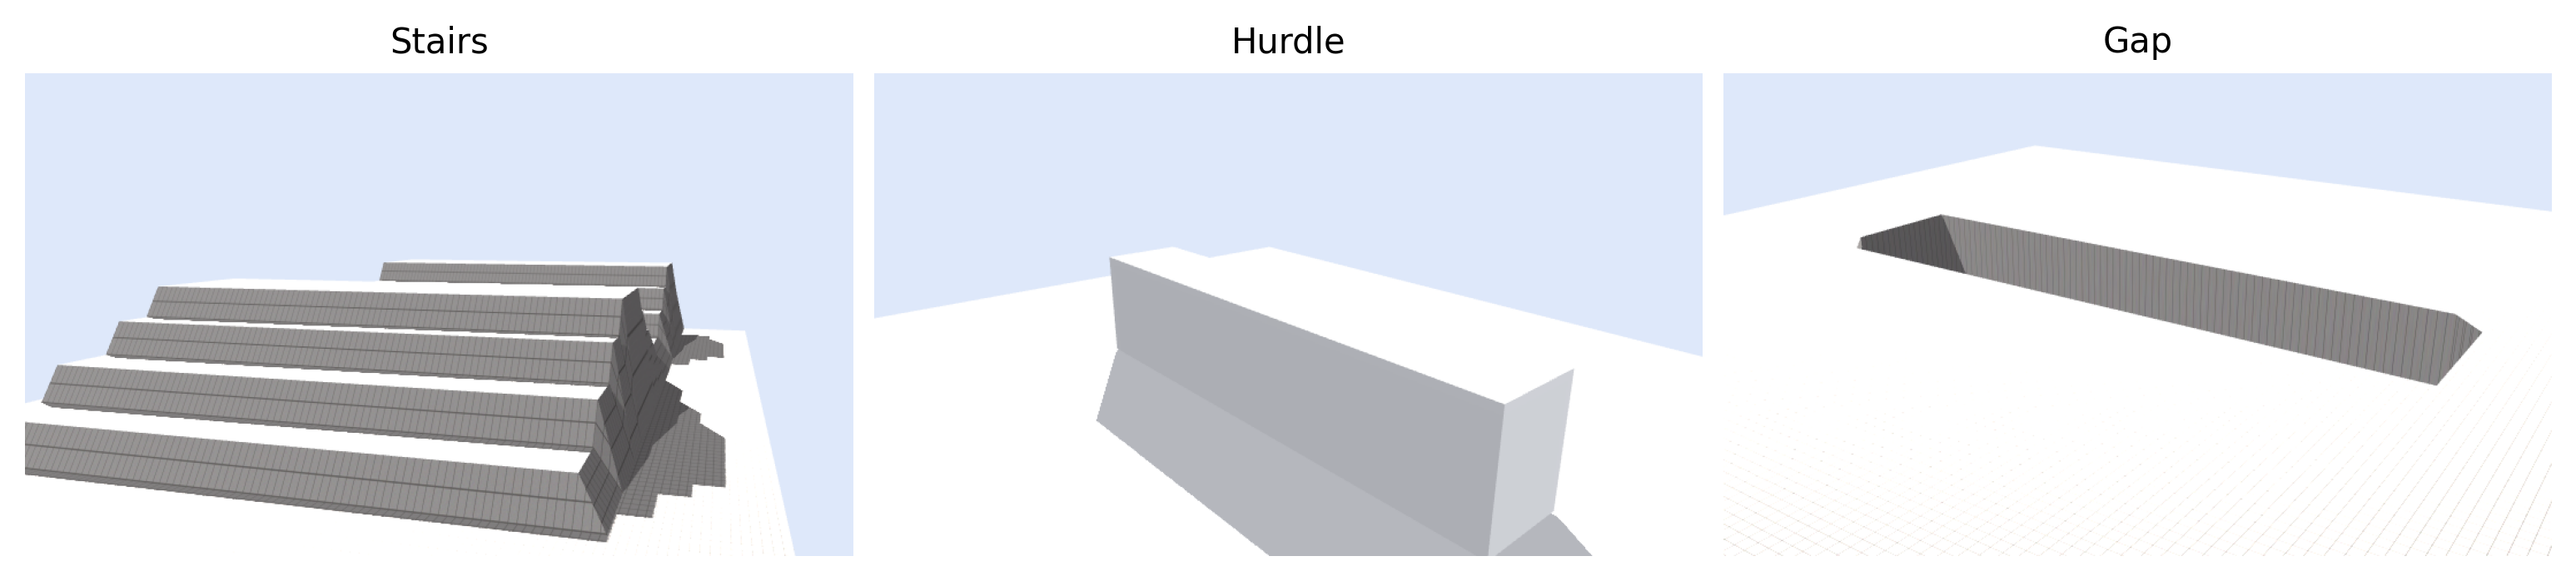
\includegraphics[width=0.94\linewidth]{parkour_obstacle_types.png}
  \end{columns}
  \source{Thesis experiments in Genesis + legged\_gym; parkour setup adapted from recent quadruped parkour work.}
\end{frame}

% Script:
% - Model the task as a POMDP so the talk has the right mathematical frame from the start.
% - The key split is proprioception plus exteroception, with different exteroception for teacher and student.
% - Emphasize that the student only gets partial information, so recurrence is not cosmetic; it is motivated by the model.
% - Transition: with the task defined, the next question is how the policy is learned.
\begin{frame}{Mathematical Setup}
  \begin{columns}[T,onlytextwidth]
    \column{0.56\textwidth}
    \small
    We model parkour as a POMDP
    \[
      (\mathcal{S}, \mathcal{A}, \mathcal{O}, T, R, \gamma),
      \qquad
      J(\pi) = \E_{\pi}\!\left[\sum_{t=0}^{\infty} \gamma^t R(s_t,a_t)\right].
    \]

    \begin{itemize}
      \item Actions are joint target offsets: \(a_t \in \R^{12}\).
      \item Observations split as \(o_t = (o_{\mathrm{prop}}, o_{\mathrm{ext}})\).
      \item \(o_{\mathrm{prop}} \in \R^{53}\): IMU, commands, joint states, previous actions, foot contacts.
      \item \(o_{\mathrm{ext}}\): \alert{scandot heightmaps} for the teacher, or a \alert{monocular depth image} for the student.
    \end{itemize}

    \column{0.40\textwidth}
    \begin{block}{Teacher Observation}
      \[
        o^{T}_t = \bigl(o_{\mathrm{prop}},\ \text{scandots},\ \text{priv.\ params}\bigr)
      \]
      Direct terrain geometry during training.
    \end{block}

    \begin{block}{Student Observation}
      \[
        o^{S}_t = \bigl(o_{\mathrm{prop}},\ \text{depth image}\bigr)
      \]
      Partial observation, so a recurrent encoder is justified.
    \end{block}
  \end{columns}
\end{frame}

% ==========================================================================
\section{Method}
% ==========================================================================

\sectionslide{QueensGold}{Method}

% Script:
% - This is the high-level pipeline slide.
% - Stage 1 learns a strong teacher from privileged terrain geometry.
% - Stage 2 distills that behavior into a student that only sees proprioception plus depth.
% - Transition: after the pipeline, I will briefly define the two optimization objectives.
\begin{frame}{Two-Stage Learning Pipeline}
  \begin{columns}[T,onlytextwidth]
    \column{0.54\textwidth}
    \centering
    \scalebox{0.78}{% Pipeline diagram: two-stage teacher-student distillation
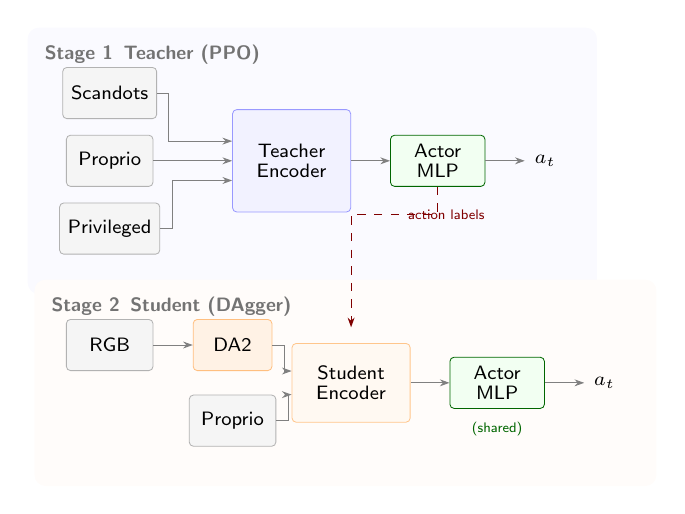
\begin{tikzpicture}[
  >=Stealth,
  % --- shared block base ---
  blkbase/.style={
    rounded corners=1.5pt, minimum height=6.5mm,
    inner xsep=3pt, inner ysep=1.5pt,
    line width=0.3pt, align=center, font=\scriptsize\sffamily
  },
  % --- block types ---
  inp/.style={blkbase, draw=black!30, fill=gray!8, minimum width=11mm},
  da2/.style={blkbase, draw=orange!50, fill=orange!10, minimum width=10mm},
  tenc/.style={blkbase, draw=blue!40, fill=blue!5, minimum width=15mm, minimum height=13mm},
  senc/.style={blkbase, draw=orange!45, fill=orange!5, minimum width=15mm, minimum height=10mm},
  act/.style={blkbase, draw=green!40!black, fill=green!5, minimum width=12mm},
  % --- labels ---
  outlbl/.style={font=\scriptsize\sffamily},
  stglbl/.style={font=\scriptsize\sffamily\bfseries, text=black!55, anchor=north west},
  annot/.style={font=\tiny\sffamily},
  % --- arrows ---
  arr/.style={-{Stealth[length=3.5pt, width=2.5pt]}, line width=0.35pt, draw=black!50},
  darr/.style={-{Stealth[length=3.5pt, width=2.5pt]}, line width=0.4pt, dashed, draw=red!50!black},
]

% ===================== STAGE 1: TEACHER =====================

\node[inp] (scan) at (0, 0) {Scandots};
\node[inp, below=2mm of scan] (prop1) {Proprio};
\node[inp, below=2mm of prop1] (priv) {Privileged};

\node[tenc, right=10mm of prop1] (te) {Teacher\\[-1pt]Encoder};
\node[act] (ta) at ([xshift=11mm]te.east) {Actor\\[-1pt]MLP};
\node[outlbl, right=5mm of ta] (tout) {$a_t$};

\draw[arr] (scan.east) -- ++(1.5mm,0) |- ([yshift=2.5mm]te.west);
\draw[arr] (prop1) -- (te);
\draw[arr] (priv.east) -- ++(1.5mm,0) |- ([yshift=-2.5mm]te.west);
\draw[arr] (te) -- (ta);
\draw[arr] (ta) -- (tout);

% Stage 1 background
\begin{scope}[on background layer]
  \node[draw=none, fill=blue!2, rounded corners=4pt,
    fit=(scan)(priv)(tout), inner xsep=4mm, inner ysep=5mm] (s1) {};
  \node[stglbl] at ([xshift=1mm, yshift=-1mm]s1.north west)
    {Stage 1\enspace Teacher (PPO)};
\end{scope}

% ===================== STAGE 2: STUDENT =====================

\node[inp] (rgb) at (0, -3.2) {RGB};
\node[da2, right=5mm of rgb] (d2) {DA2};
\node[inp, below=3mm of d2] (prop2) {Proprio};

\node[senc] (se) at ([xshift=10mm]d2.east |- {$(d2)!0.5!(prop2)$}) {Student\\[-1pt]Encoder};
\node[act] (sa) at ([xshift=11mm]se.east) {Actor\\[-1pt]MLP};
\node[outlbl, right=5mm of sa] (sout) {$a_t$};

\draw[arr] (rgb) -- (d2);
\draw[arr] (d2.east) -- ++(1.5mm,0) |- ([yshift=1.5mm]se.west);
\draw[arr] (prop2.east) -- ++(1.5mm,0) |- ([yshift=-1.5mm]se.west);
\draw[arr] (se) -- (sa);
\draw[arr] (sa) -- (sout);

% Stage 2 background
\begin{scope}[on background layer]
  \node[draw=none, fill=orange!2, rounded corners=4pt,
    fit=(rgb)(prop2)(sout), inner xsep=4mm, inner ysep=5mm] (s2) {};
  \node[stglbl] at ([xshift=1mm, yshift=-1mm]s2.north west)
    {Stage 2\enspace Student (DAgger)};
\end{scope}

% ===================== CONNECTIONS =====================

% DAgger supervision arrow
\draw[darr]
  (ta.south) -- ++(0,-3.5mm)
  -| node[pos=0.25, right=0.5mm, annot, text=red!50!black] {action labels}
  ([yshift=2mm]se.north);

% Shared actor annotation
\node[annot, text=green!40!black, below=0.5mm of sa] {(shared)};

\end{tikzpicture}
}

    \column{0.42\textwidth}
    \small
    \begin{enumerate}
      \item \textbf{Teacher:} PPO with privileged scandot geometry and randomized physics.
      \item \textbf{Student:} DAgger distillation on the \emph{student's} state distribution.
      \item \textbf{Deployment question:} replace simulator depth with DA2-estimated monocular depth.
    \end{enumerate}

    \vspace{0.2em}
    \begin{block}{Why this pipeline?}
      It separates two bottlenecks:
      \begin{itemize}
        \item \textbf{Control:} can a depth-based student act at all?
        \item \textbf{Perception:} does monocular depth preserve enough geometry?
      \end{itemize}
    \end{block}
  \end{columns}
  \source{Pipeline adapted from the thesis; PPO after Schulman et al. (2017), DAgger after Ross et al. (2011).}
\end{frame}

% Script:
% - I only need to define what is optimized, not teach an RL course.
% - For PPO, the main point is stable policy improvement through clipping.
% - For DAgger, the main point is imitation on the student's own state distribution.
% - Transition: once the control side is defined, I can explain the monocular depth side and DSQ.
\begin{frame}{Training Objectives}
  \begin{columns}[T,onlytextwidth]
    \column{0.49\textwidth}
    \begin{block}{Teacher: PPO}
      \footnotesize
      \[
        L^{\mathrm{CLIP}}
        =
        \E_t\!\left[
          \min\!\left(
            r_t \hat{A}_t,\;
            \clip(r_t,1-\epsilon,1+\epsilon)\hat{A}_t
          \right)
        \right]
      \]
      \begin{itemize}
        \item Large updates can collapse performance.
        \item Clipping keeps policy improvement conservative.
      \end{itemize}
    \end{block}

    \column{0.49\textwidth}
    \begin{block}{Student: DAgger}
      \footnotesize
      \[
        \mathcal{L}
        =
        \|a_{\mathrm{teacher}} - a_{\mathrm{student}}\|_2
        +
        \|y_{\mathrm{oracle}} - \hat{y}\|_2
      \]
      \begin{itemize}
        \item Student predicts actions from proprioception + depth.
        \item Teacher actions are executed, so labels stay reliable while the student explores.
      \end{itemize}
    \end{block}
  \end{columns}

  \vspace{0.2em}
  \begin{alertblock}{Takeaway}
    The teacher solves the control problem first; the student then isolates the perception-to-action transfer problem.
  \end{alertblock}
\end{frame}

% Script:
% - This is the main math contribution slide.
% - DA2 gives a depth map from one RGB image, but monocular depth is only defined up to scale and shift.
% - That is why DSQ is a correlation metric rather than an absolute depth error.
% - Transition: with the metric defined, I can show what the experiments say.
\begin{frame}{Monocular Depth and Depth Signal Quality}
  \begin{columns}[T,onlytextwidth]
    \column{0.58\textwidth}
    \small
    Monocular depth estimation maps
    \[
      I \in \R^{H \times W \times 3}
      \;\mapsto\;
      \hat d = f_{\phi}(I) \in \R^{H \times W}.
    \]

    To measure whether estimated depth preserves terrain geometry, I define
    \[
      \DSQ
      =
      \frac{1}{T} \sum_{t=1}^{T}
      \frac{1}{N} \sum_{i=1}^{N}
      \rho\!\left(d_i^{\mathrm{GT}}, d_i^{\mathrm{DA2}}\right),
    \]
    where \(\rho\) is Pearson correlation over image pixels.

    \column{0.38\textwidth}
    \begin{block}{Why correlation?}
      \[
        \rho(\alpha x + \beta,\ y) = \rho(x,y),
        \qquad \alpha > 0
      \]
      so DSQ is insensitive to the scale--shift ambiguity inherent in monocular depth.
    \end{block}

    \begin{block}{Interpretation}
      \begin{itemize}
        \item \textbf{High DSQ:} terrain shape is preserved.
        \item \textbf{Low DSQ:} geometry is being lost before control even acts.
      \end{itemize}
    \end{block}
  \end{columns}
  \source{DA2 after Yang et al. (2024); DSQ defined in the thesis as a geometry-preservation diagnostic.}
\end{frame}

% ==========================================================================
\section{Results}
% ==========================================================================

\sectionslide{QueensRed}{Results}

% Script:
% - Start with the ceiling to avoid over-interpreting later failures.
% - The teacher is nearly perfect, and the GT-depth student is strong across all gap rows.
% - The zero-depth ablation is important because it rules out the idea that the student is just using proprioceptive heuristics.
% - Transition: now I can replace GT depth with DA2 depth and see where performance degrades.
\begin{frame}{Baselines Establish the Ceiling}
  \begin{columns}[T,onlytextwidth]
    \column{0.47\textwidth}
    \centering
    \small
    \begin{tabular}{@{}lcccc@{}}
      \toprule
      & R0 & R1 & R2 & R3 \\
      \midrule
      Teacher & 98.5 & 100.0 & 99.0 & 98.5 \\
      GT-depth & 94.5 & 94.5 & 89.1 & 87.5 \\
      Zero-depth & 8.0 & 2.0 & 0.0 & 0.0 \\
      \bottomrule
    \end{tabular}

    \vspace{0.4em}
    \footnotesize Gap-course success rate (\%).

    \column{0.49\textwidth}
    \begin{block}{What this tells us}
      \begin{itemize}
        \item The \alert{student architecture is capable}: one depth view plus recurrence is enough to act.
        \item The main bottleneck is \alert{depth quality}, not the downstream controller.
        \item Removing depth almost completely destroys performance.
      \end{itemize}
    \end{block}

    \begin{alertblock}{Interpretation}
      If monocular depth fails later, that failure should be attributed mainly to the \emph{perception pipeline}, not to the control stack.
    \end{alertblock}
  \end{columns}
\end{frame}

% Script:
% - This is the core empirical result slide.
% - DA2-small is not enough, DA2-base helps, and adding texture closes much of the remaining gap.
% - The image panel makes the mechanism intuitive: featureless gaps are hard because the boundary is weak in RGB, so DA2 has less geometry to recover.
% - Transition: the next slide asks whether this behavior generalizes across appearance changes, and whether DSQ predicts failure.
\begin{frame}{Estimated Depth: Model Size and Texture Matter}
  \begin{columns}[T,onlytextwidth]
    \column{0.46\textwidth}
    \centering
    \small
    \begin{tabular}{@{}lcccc@{}}
      \toprule
      Configuration & R0 & R1 & R2 & R3 \\
      \midrule
      DA2-small & 56.3 & 33.6 & --- & --- \\
      DA2-base & 68.4 & 83.2 & 26.6 & 0.8 \\
      DA2-base + texture & 64.8 & 64.1 & 68.0 & 44.9 \\
      \midrule
      GT-depth & 94.5 & 94.5 & 89.1 & 87.5 \\
      \bottomrule
    \end{tabular}

    \vspace{0.5em}
    \begin{itemize}
      \item Larger depth models help.
      \item Texture especially helps \alert{gaps}.
      \item Hard rows remain unsolved.
    \end{itemize}

    \column{0.50\textwidth}
    \centering
    \begin{tabular}{cc}
      \scriptsize Untextured & \scriptsize Checkerboard \\
      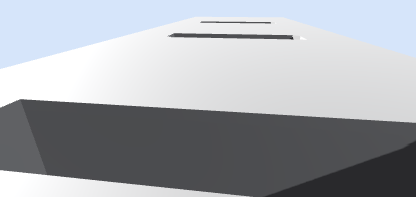
\includegraphics[width=0.47\linewidth]{gap_untextured_rgb.png} &
      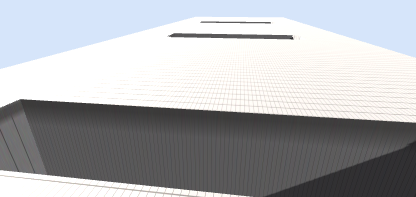
\includegraphics[width=0.47\linewidth]{gap_textured_rgb.png} \\
      \scriptsize DA2 output & \scriptsize DA2 output \\
      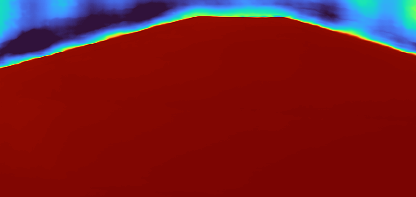
\includegraphics[width=0.47\linewidth]{gap_untextured_da2.png} &
      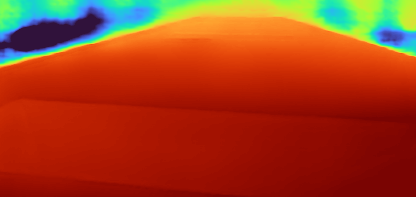
\includegraphics[width=0.47\linewidth]{gap_textured_da2.png} \\
    \end{tabular}

    \vspace{0.4em}
    \footnotesize Featureless terrain weakens the visual cue that defines the gap boundary.
  \end{columns}
\end{frame}

% Script:
% - This slide ties the experiments back to the math through DSQ.
% - The student is fairly tolerant to moderate lighting and color changes, but not to featureless surfaces or some unseen textures.
% - DSQ is useful because low DSQ often coincides with failure, but it is not a complete predictor.
% - Transition: I’ll close with what these experiments actually taught me.
\begin{frame}{Sensitivity Study and the Role of DSQ}
  \begin{columns}[T,onlytextwidth]
    \column{0.54\textwidth}
    \centering
    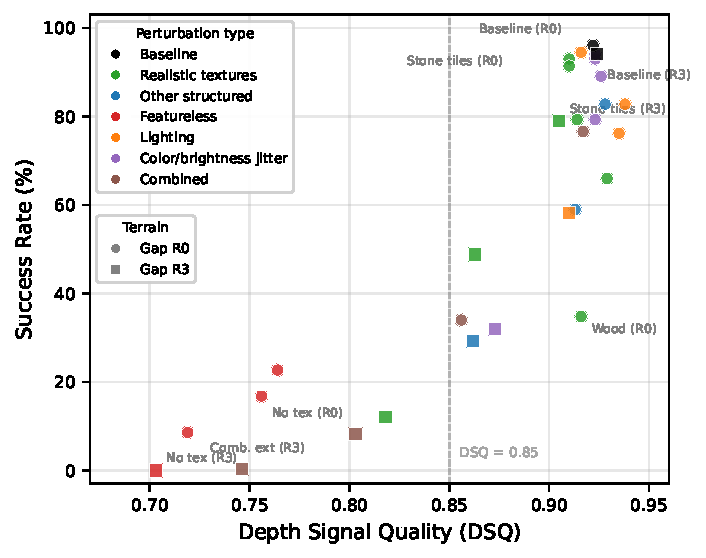
\includegraphics[width=0.96\linewidth]{dsq_scatter.pdf}

    \column{0.42\textwidth}
    \small
    \begin{block}{Appearance perturbations}
      \begin{itemize}
        \item Realistic texture replacements
        \item Featureless or noisy surfaces
        \item Brightness, color, and combined shifts
      \end{itemize}
    \end{block}

    \begin{alertblock}{Main pattern}
      \begin{itemize}
        \item Lighting and color changes are often tolerable.
        \item Featureless surfaces produce the largest failures.
        \item High DSQ helps, but \alert{does not guarantee} success.
      \end{itemize}
    \end{alertblock}
  \end{columns}
  \source{DSQ-vs-success scatter computed over six terrain settings and multiple test-time perturbation categories.}
\end{frame}

% Script:
% - I want this slide to sound intellectually honest rather than promotional.
% - The strongest claims are about what the experiments support, and what they rule out.
% - This is the slide that makes the thesis feel like a self-directed mathematical investigation rather than just a benchmark report.
% - Transition: I’ll end by being explicit about the limitations and the next step.
\begin{frame}{What the Experiments Ruled In and Ruled Out}
  \begin{columns}[T,onlytextwidth]
    \column{0.48\textwidth}
    \begin{block}{Ruled In}
      \begin{itemize}
        \item Monocular depth can support \alert{nontrivial parkour in simulation}.
        \item The teacher--student pipeline is a useful way to isolate perception from control.
        \item DSQ is a meaningful \alert{failure indicator} when geometry collapses.
      \end{itemize}
    \end{block}

    \column{0.48\textwidth}
    \begin{alertblock}{Ruled Out / Still Open}
      \begin{itemize}
        \item Success is \alert{not} explained by proprioceptive heuristics alone.
        \item Monocular depth is \alert{not yet robust enough} for hard, texture-poor cases.
        \item Real-world transfer remains open; the thesis is a proof of concept, not a deployment claim.
      \end{itemize}
    \end{alertblock}
  \end{columns}

  \vspace{0.2em}
  \begin{block}{Bottom line}
    The main contribution is methodological and experimental: it identifies \emph{where} monocular depth helps, \emph{where} it breaks, and \emph{why} geometry preservation matters.
  \end{block}
\end{frame}

% ==========================================================================
\section{Conclusion}
% ==========================================================================

% Script:
% - End with limitations first, then the next step, so the final tone is honest but forward-looking.
% - The key message is that this is a credible proof of concept with clear bottlenecks.
% - If time is tight, the only sentence I need to land is: perception quality, not control, is the limiting factor.
\begin{frame}{Limitations and Next Step}
  \begin{columns}[T,onlytextwidth]
    \column{0.48\textwidth}
    \begin{block}{Limitations}
      \begin{itemize}
        \item All results are in \alert{simulation only}.
        \item Obstacles are simpler than the hardest recent parkour benchmarks.
        \item DA2 is still brittle on weak-texture surfaces.
        \item DSQ explains many failures, but not all of them.
        \item The current perception stack is too heavy for onboard deployment.
      \end{itemize}
    \end{block}

    \column{0.48\textwidth}
    \begin{block}{Next Step}
      \begin{itemize}
        \item Hardware evaluation on Unitree Go2.
        \item Smaller or temporally consistent depth models.
        \item Broader testing on harder courses and outdoor conditions.
        \item Possibly adapt the perception model and policy jointly.
      \end{itemize}
    \end{block}
  \end{columns}

  \vspace{0.2em}
  \begin{alertblock}{Final message}
    The experiments suggest that \alert{perception quality}, not the student controller, is the dominant bottleneck in monocular parkour.
  \end{alertblock}
\end{frame}

% ==========================================================================
% CLOSING
% ==========================================================================

\sectionslide{QueensBlue}{Thank you! \\[1em]Questions?}

% ==========================================================================
% BACKUP SLIDES
% ==========================================================================

\appendix
\section{Backup}

% Script:
% - Use this only if someone asks what the recurrent student actually looks like.
% - The key point is that recurrence produces a latent terrain representation and a heading estimate from depth plus proprioception.
\begin{frame}{Backup: Student Architecture}
  \begin{columns}[T,onlytextwidth]
    \column{0.58\textwidth}
    \centering
    \scalebox{0.92}{% Student visual encoder architecture
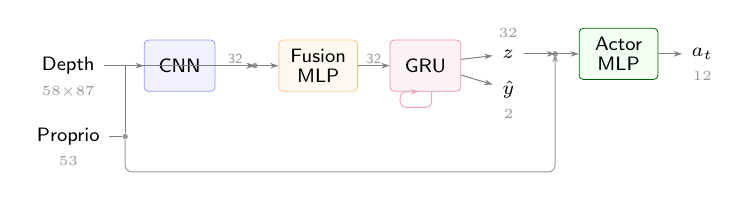
\begin{tikzpicture}[
  >=Stealth,
  % --- shared block base ---
  blkbase/.style={
    rounded corners=1.5pt, minimum height=6.5mm,
    inner xsep=2.5pt, inner ysep=1.5pt,
    line width=0.3pt, align=center, font=\scriptsize\sffamily
  },
  % --- block types ---
  cnn/.style={blkbase, draw=blue!40, fill=blue!5, minimum width=9mm},
  fuse/.style={blkbase, draw=orange!45, fill=orange!5, minimum width=10mm},
  gru/.style={blkbase, draw=purple!40, fill=purple!5, minimum width=9mm},
  act/.style={blkbase, draw=green!40!black, fill=green!5, minimum width=10mm},
  % --- labels ---
  io/.style={font=\scriptsize\sffamily},
  dim/.style={font=\tiny\sffamily, text=black!40, inner sep=0.5pt},
  % --- arrows ---
  arr/.style={-{Stealth[length=3pt, width=2pt]}, line width=0.35pt, draw=black!50},
]

% ===================== INPUTS =====================

\node[io] (depth) at (0, 0.4) {Depth};
\node[dim, below=0mm of depth] {$58{\times}87$};

\node[io] (prop) at (0, -0.5) {Proprio};
\node[dim, below=0mm of prop] {$53$};

% ===================== PROCESSING =====================

\node[cnn, right=5mm of depth] (cnn) {CNN};

% Concat point 1
\coordinate (cat1) at ([xshift=5mm]cnn.east);
\node[circle, fill=black!40, inner sep=0.7pt] at (cat1) {};

\node[fuse, right=3mm of cat1] (fmlp) {Fusion\\[-1pt]MLP};

\node[gru, right=4mm of fmlp] (gru) {GRU};

% GRU recurrence
\draw[arr, rounded corners=2pt, draw=purple!35]
  ([xshift=0.8mm]gru.south) -- ++(0,-2mm) -- ++(-4mm,0) -- ++(0,2mm)
  -- ([xshift=-0.8mm]gru.south);

% ===================== GRU OUTPUTS =====================

\node[io, right=4mm of gru, yshift=1.5mm] (z) {$z$};
\node[dim, above=0mm of z] {$32$};
\node[io, right=4mm of gru, yshift=-3mm] (yhat) {$\hat{y}$};
\node[dim, below=0mm of yhat] {$2$};

% Concat point 2
\coordinate (cat2) at ([xshift=4mm]z.east);
\node[circle, fill=black!40, inner sep=0.7pt] at (cat2) {};

\node[act, right=3mm of cat2] (actor) {Actor\\[-1pt]MLP};

\node[io, right=3mm of actor] (out) {$a_t$};
\node[dim, below=0mm of out] {$12$};

% ===================== ARROWS =====================

\draw[arr] (depth) -- (cnn);
\draw[arr] (cnn) -- node[dim, above] {32} (cat1);
\draw[arr] (cat1) -- (fmlp);
\draw[arr] (fmlp) -- node[dim, above] {32} (gru);
\draw[arr] ([yshift=0.8mm]gru.east) -- (z);
\draw[arr] ([yshift=-1.2mm]gru.east) -- (yhat);
\draw[arr] (z) -- (cat2);
\draw[arr] (cat2) -- (actor);
\draw[arr] (actor) -- (out);

% Proprio branch point
\node[circle, fill=black!40, inner sep=0.7pt] (pbr) at ([xshift=2mm]prop.east) {};

% Branch 1: to fusion
\draw[arr] (prop.east) -- (pbr) |- (cat1);

% Branch 2: to actor (route below)
\draw[arr, rounded corners=2.5pt, draw=black!40]
  (pbr) -- ++(0,-4.5mm) -| (cat2);

\end{tikzpicture}
}

    \column{0.38\textwidth}
    \begin{itemize}
      \item CNN encodes the \(58 \times 87\) depth image.
      \item Proprioception is fused before the GRU.
      \item The GRU outputs a terrain latent \(z \in \R^{32}\) and heading estimate \(\hat y \in \R^2\).
      \item The teacher's actor MLP is reused downstream.
    \end{itemize}
  \end{columns}
\end{frame}

% Script:
% - This slide is for technical questions about the optimization setup.
% - I do not need every coefficient; I only need enough to show the design was deliberate.
\begin{frame}{Backup: Reward and Training Details}
  \begin{columns}[T,onlytextwidth]
    \column{0.48\textwidth}
    \begin{block}{Teacher Reward Structure}
      \small
      \begin{itemize}
        \item Task progress: velocity, heading, course progress, success bonus
        \item Termination and collision penalties
        \item Locomotion regularization: torque, power, action smoothness
        \item Body stability: orientation, angular velocity, flat back
      \end{itemize}
    \end{block}

    \begin{block}{Control}
      \begin{itemize}
        \item 12 actuated joints
        \item 50 Hz action rate
        \item PD control with \(K_p = 30.0\), \(K_d = 0.75\)
      \end{itemize}
    \end{block}

    \column{0.48\textwidth}
    \begin{block}{Key PPO Hyperparameters}
      \small
      \begin{tabular}{@{}lr@{}}
        \toprule
        Environments & 4096 \\
        LR & \(10^{-3}\) \\
        \(\gamma\) & 0.99 \\
        \(\lambda\) & 0.95 \\
        Clip \(\epsilon\) & 0.2 \\
        \bottomrule
      \end{tabular}
    \end{block}

    \begin{block}{Key DAgger Hyperparameters}
      \small
      \begin{tabular}{@{}lr@{}}
        \toprule
        Environments & 48 \\
        BPTT window & 24 \\
        LR & \(2 \times 10^{-3}\) \\
        Actor LR scale & 0.1 \\
        \bottomrule
      \end{tabular}
    \end{block}
  \end{columns}
\end{frame}

% Script:
% - This is the visual backup for the texture argument.
% - It is useful if someone asks what the depth model is actually seeing across surfaces.
\begin{frame}{Backup: Qualitative Visual Examples}
  \centering
  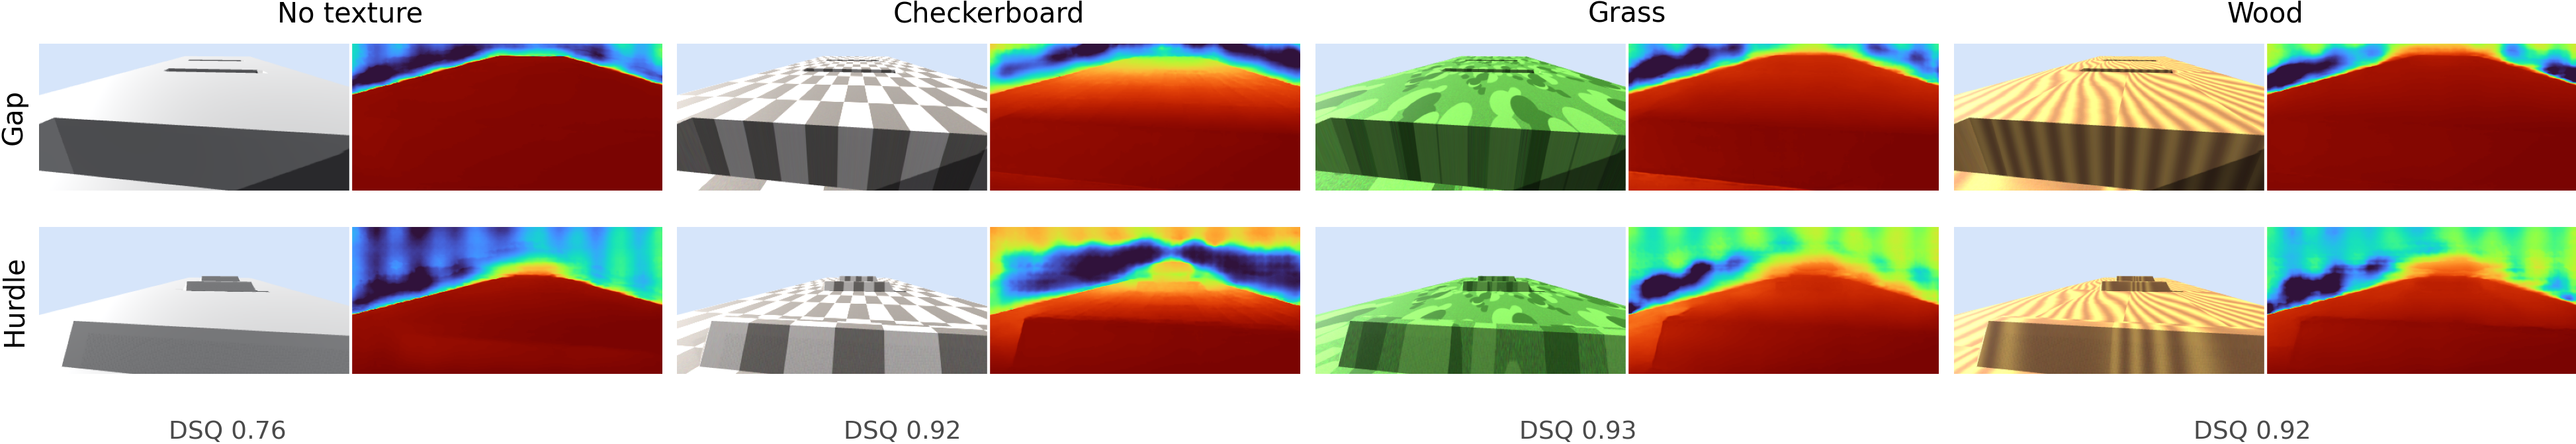
\includegraphics[width=0.93\linewidth]{da2_texture_comparison.png}

  \vspace{0.4em}
  \small
  Featureless terrain produces the weakest obstacle localization; structured textures preserve substantially more geometry.
\end{frame}

\end{document}
